\documentclass{beamer}
\usepackage[utf8]{inputenc}
\usepackage[T1]{fontenc}
\usepackage{textcomp}
%\usepackage{amsmath,amssymb,lmodern}
%\usepackage{mathptmx}
%\usepackage[scaled=.90]{helvet}
%\usepackage{courier}
\usetheme[titleformat=allcaps,block=fill]{metropolis}
\title{Card Layout Interpretation}
\subtitle{Alogorithm to interpret sequence process models}
\date{\today}
\author{Thomas Fragner}
\institute{Centre for Modern Beamer Themes}
\begin{document}
  \maketitle
  \section{First Section}
  \begin{frame}{First Frame}
    \begin{alertblock}{This is an Alert block}
     This is an important alert
     \end{alertblock}
  \end{frame}
  \section{Second Section}
  \begin{frame}[standout]
  Thank you! \end{frame}
  \begin{frame}{First Frame}
	  In this slide, some important text will be
	  \alert{highlighted} beause it's important.
	  Please, don't abuse it.
 
	  \begin{block}{Remark}
	  Sample text
	  \end{block}
 
	  \begin{alertblock}{Important theorem}
	  Sample text in red box
	  \end{alertblock}
 
	  \begin{examples}
	  Sample text in green box. "Examples" is fixed as block title.
	  \end{examples}
  \end{frame}
  \section{Third Section}
  \begin{frame}{First Frame}
	\frametitle{A frame}
	\begin{columns}
		\column{0.5\textwidth}
	  	\begin{figure}[h]
	     \centering	
	     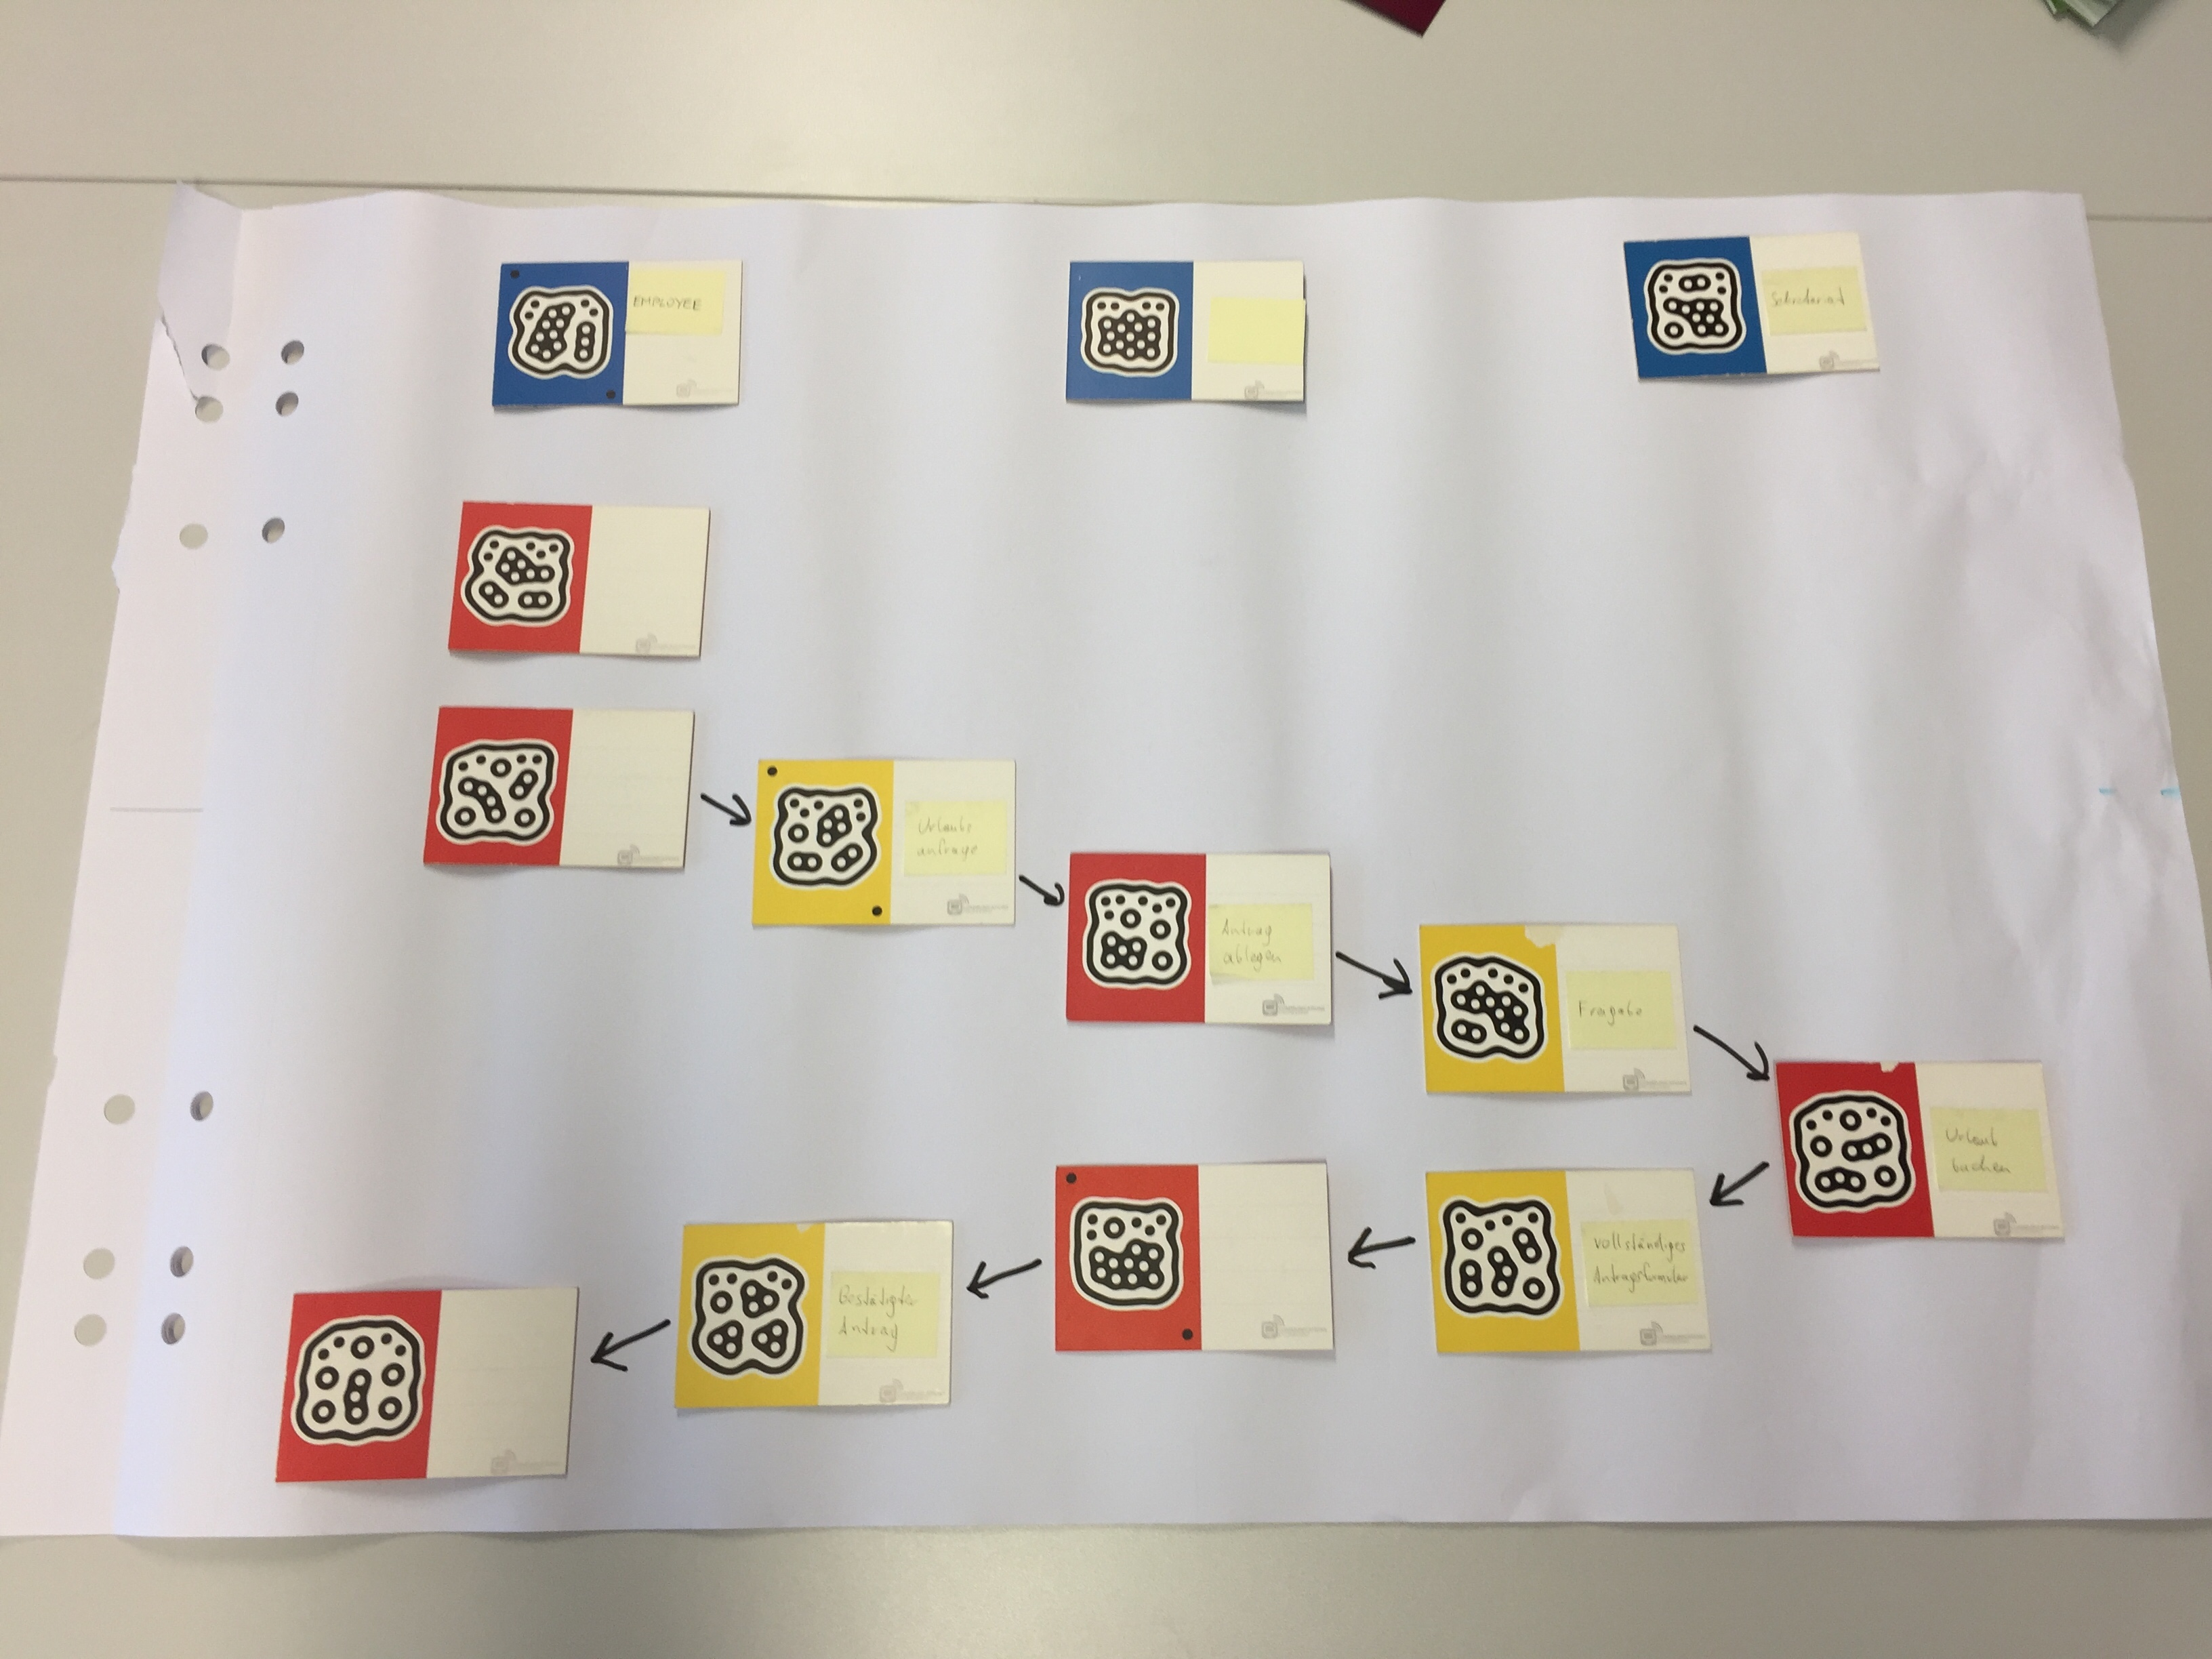
\includegraphics[width=.9\textwidth]{figures/linienlegemethode.jpg}
	     \caption{caption}
	     \label{fig:figures_linienlegemethode}
	    \end{figure}
	  \column{0.5\textwidth}
	  \begin{itemize}
		  \item teasdfasdf
		  \item asdfasdfasd
		 \end{itemize}
	  \end{columns}
  \end{frame}
  \section{Forth Section}
  \begin{frame}{First Frame}
	\frametitle{Two-column slide}
 
	\begin{columns}
 
	\column{0.5\textwidth}
	This is a text in first column.
	$$E=mc^2$$
	\begin{itemize}
	\item First item
	\item Second item
	\end{itemize}
 
	\column{0.5\textwidth}
	This text will be in the second column
	and on a second tought this is a nice looking
	layout in some cases.
	\end{columns}
  \end{frame}
  \begin{frame}[label=conclusion, standout]{Conclusion} Awesome slide
  \end{frame}
\end{document}
